\documentclass[12pt]{article}
\usepackage{amsmath}
\usepackage{hyperref}
\usepackage{verbatim}
\usepackage{graphicx}
\begin{document}
\subsection{Boris Algorithm}
This code is a modification of the code presented in this \href{https://www.youtube.com/watch?v=d4NlmGkfagk&t=889s&ab_channel=PyPhy}{video}. The derivation of the algorithm will be taken from \href{http://www.amazon.com/gp/product/0750310251/ref=as_li_ss_tl?ie=UTF8&tag=slovcook-20&linkCode=as2&camp=217145}{Birdsall's book}, unless otherwise mentioned everything is sourced from there\cite{Birdsall}.
The particle equations of motion to be integrated are (assuming no force outside of electric and magnetic): 
$$\frac{d\textbf{v}}{dt}=\frac{q}{m}\left(\textbf{E}+\textbf{v}\wedge\textbf{B}\right)$$
$$\frac{d\textbf{x}}{dt}=\textbf{v}$$
We want a centered difference scheme, and we do this by evaluating the velocity vector at half-steps:
\begin{equation}\label{discretlorenz}
\frac{\textbf{v}_{t+\Delta t/2}-\textbf{v}_{t-\Delta t/2}}{\Delta t}=\frac{q}{m}\left(\textbf{E}+\frac{\textbf{v}_{t+\Delta t/2}+\textbf{v}_{t-\Delta t/2}}{2}\wedge\textbf{B}\right)
\end{equation}
The Boris algorithm introduces new velocity variables to separate the solution steps of the magnetic and electric fields:
\begin{equation}\label{v+v-}
\begin{split}
\textbf{v}^-=\textbf{v}_{t-\Delta t/2}+\frac{q\textbf{E}}{m}\frac{\Delta t}{2}\\
\textbf{v}^+=\textbf{v}_{t+\Delta t/2}-\frac{q\textbf{E}}{m}\frac{\Delta t}{2}
\end{split}
\end{equation}
Plugging this into \eqref{discretlorenz} yields
\begin{equation}\label{discretboris}
\frac{\textbf{v}^+-\textbf{v}^-}{\Delta t}=\frac{q}{2m}(\textbf{v}^++\textbf{v}^-)\wedge\textbf{B}
\end{equation}
This is a pure rotation of $\textbf{v}$. To show this, let's take the dot product of \eqref{discretboris} with $(\textbf{v}^++\textbf{v}^-)$, doing this cancels out the RHS because the dot product of perpendicular vectors is zeros, so we get
$$\textbf{v}^+\cdot(\textbf{v}^++\textbf{v}^-)=\textbf{v}^-\cdot(\textbf{v}^++\textbf{v}^-)$$
Taking advantage of the commutative nature of the dot product we get
$$|v^+|^2=|v^-|^2$$
Since $\textbf{v}^+$ is the time evolution of $\textbf{v}^-$ the only thing that \eqref{discretboris} can change is orientation, and thus it is only a rotation. Therefore, if we know what angle is traversed we can use rotation matrices in the solution process. In fact the solution process is the following:
\begin{itemize}
\item Add half the electric impulse to $\textbf{v}_{t-\Delta t/2}$ via \eqref{v+v-} to obtain $\textbf{v}^-$
\item Rotate through the angle dictated by \eqref{discretboris} to get $\textbf{v}^+$
\item Add the remaining half of the electric impulse to $\textbf{v}^+$ to obtain $\textbf{v}_{t+\Delta t/2}$
\end{itemize}
Now we need to derive the angle by which the velocity is rotated, we can do it by drawing the following figure:

\hspace{-2cm}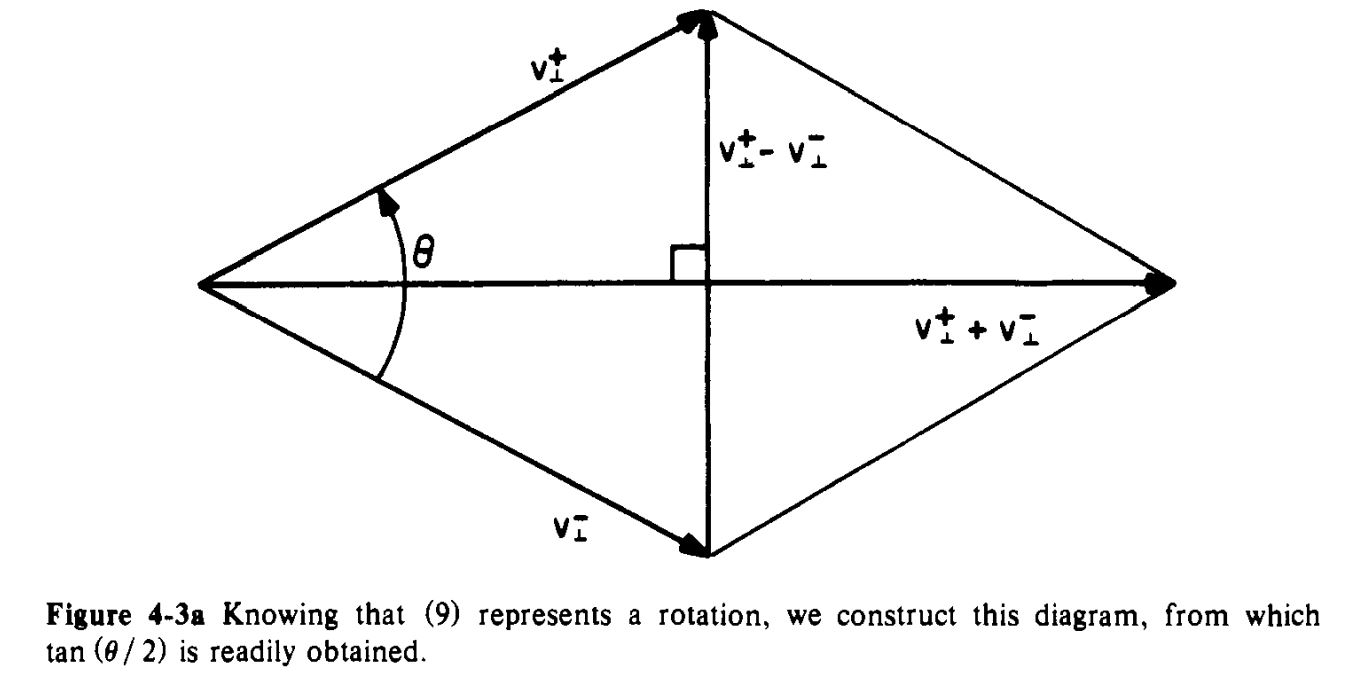
\includegraphics[scale=0.5]{anglerotated}
By construction, if we take half of $\textbf{v}^+_{\perp}-\textbf{v}^-_{\perp}$ and $\textbf{v}^+_{\perp}+\textbf{v}^-_{\perp}$ we get the legs of the right triangle in the upper left, and therefore:
$$tan\left(\frac{\theta}{2}\right)=\frac{|\textbf{v}^+_{\perp}-\textbf{v}^-_{\perp}|}{|\textbf{v}^+_{\perp}+\textbf{v}^-_{\perp}|}$$
We can then use \eqref{discretboris} and take the magnitude of the cross product with the components of the velocity perpendicular to $\textbf{B}$ and we get
$$\frac{|\textbf{v}^+_{\perp}-\textbf{v}^-_{\perp}|}{|\textbf{v}^+_{\perp}+\textbf{v}^-_{\perp}|}=\frac{qB\Delta t}{2m}$$
Therefore:
$$\bigg| tan\left(\frac{\theta}{2}\right)\bigg|=\frac{qB\Delta t}{2m}=\frac{\omega_c\Delta t}{2}$$
Now, by using the Lorenz force and the right hand rule, we realize that a particle gyrates with the opposite sign of the charge (if one defines counterclockwise as positive, as is customary), so we get a relative minus sign for $\theta$ and as $tan$ is an odd function we can define $t$ as
\begin{equation}\label{angleboris}
t\equiv tan\left(\frac{\theta}{2}\right)=-\frac{qB\Delta t}{2m}
\end{equation}
if we use the half angle formulas for $sin$ and $cos$ we get:
\begin{equation}\label{sandc}
\begin{split}
s\equiv -sin\theta =\frac{2t}{1+t^2}\\
c\equiv cos\theta=\frac{1-t^2}{1+t^2}
\end{split}
\end{equation}
Therefore, the rotation becomes
$$v_x^+=cv^-_x+sv^-_y$$
$$v_y^+=-sv^-_x+cv^-_y$$
We can reduce the number of multiplications involved in this system by defining a new variable:
\begin{equation}\label{Buneman}
\begin{split}
v_x'=v_x^-+v_y^-t\\
v_y^+=v_y^--v_x's\\
v_x^+=v'_x+v_y^+t
\end{split}
\end{equation} 
Boris (cite 1970 paper) generalized this to a case in which $\textbf{v}$ and $\textbf{B}$ have arbitrary directions via a cross product:
\begin{equation}\label{borisv'}
\textbf{v}'=\textbf{v}^-+\textbf{v}^-\wedge\textbf{t}
\end{equation}
By construction $\textbf{v}'$ is perpendicular to both $\textbf{B}$ and $\textbf{v}^+-\textbf{v}^+$, which means that the angle between $\textbf{v}^-$ and $\textbf{v}'$ is $\theta/2$, thus, we can draw the following figure:

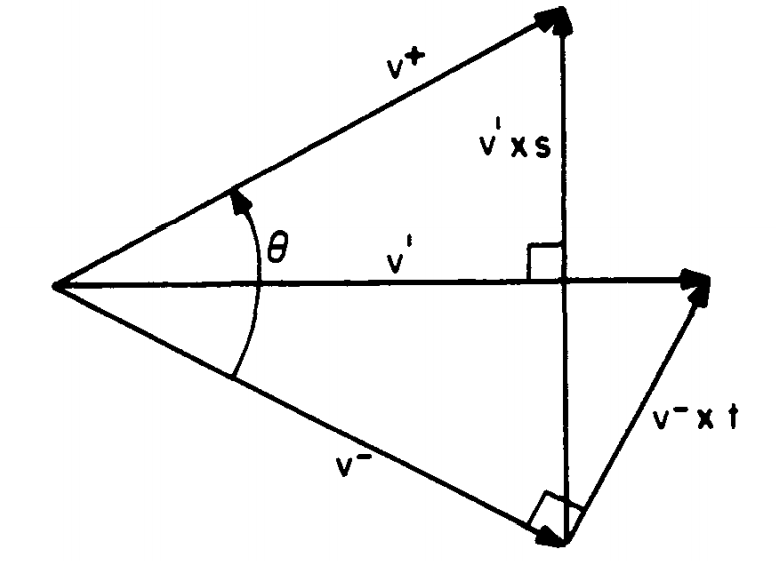
\includegraphics[scale=0.4]{vprimerot}

which shows us that 
\begin{equation}\label{tvec}
\textbf{t}\equiv-\hat{\textbf{b}}tan\left(\frac{\theta}{2}\right)=\frac{q\textbf{B}}{m}\frac{\Delta t}{2}
\end{equation}
As $\textbf{v}'$ is by construction perpendicular to both $\textbf{B}$ and $\textbf{v}^+-\textbf{v}^-$ and we are in a three-dimensional space, $\textbf{v}'\wedge\textbf{B}$ is parallel to $\textbf{v}^+-\textbf{v}^-$ and so if we define a vector $\textbf{s}$ which is parallel to $\textbf{B}$ we can make the statement:
\begin{equation}\label{borisv+}
\textbf{v}^+=\textbf{v}^-+\textbf{v}'\wedge\textbf{s}
\end{equation} 
If we take the dot product of each side we get
$$|v^+|^2=\textbf{v}^+\cdot\textbf{v}^-+\textbf{v}^+\cdot(\textbf{v}^-\wedge\textbf{s})+\textbf{v}^+\cdot(\textbf{v}^-\wedge\textbf{t})\wedge\textbf{s}$$
Let's look at just the triple product term:
$$(\textbf{v}^-\wedge\textbf{t})\wedge\textbf{s}=-\textbf{v}^-(ts)$$
Where $\textbf{v}^-\cdot\textbf{s}$ cancel because they are perpendicular. Which, when plugged into the above expression yields:
$$|v^+|^2=(1-ts)|v^-|^2cos\theta+\textbf{v}^+\cdot(\textbf{v}^-\wedge\textbf{s})=(1-ts)|v^-|^2\frac{1-t^2}{1+t^2}+\textbf{s}\cdot(\textbf{v}^+\wedge\textbf{v}^-)$$ 
Where I have used the identity derived earlier: $|v^+|^2=|v^-|^2$ as well as \eqref{sandc} and properties of the scalar product. As $\textbf{v}^+$ and $\textbf{v}^-$ form a plane, their cross product gives a vector antiparallel to $\textbf{s}$ by the right hand rule, therefore we get (again using \eqref{sandc})
$$|v^+|^2=(1-ts)|v^-|^2\frac{1-t^2}{1+t^2}-s|v^-|^2sin\theta=(1-ts)|v^-|^2\frac{1-t^2}{1+t^2}+s|v^-|^2\frac{2t}{1+t^2}$$
Pulling out a common factor:
$$|v^+|^2=|v^-|^2\frac{(1-ts)(1-t^2)+2st}{1+t^2}$$
By the fact that we want $|v^+|^2=|v^-|^2$
$$1+t^2=1+ts-t^2+st^3$$
$$2t=(1+t^2)s$$
And since $\textbf{s}$ is definitionally parallel to $\textbf{B}$ we get
\begin{equation}\label{boriss}
\textbf{s}=\frac{2\textbf{t}}{1+t^2}
\end{equation}
Finally, we can combine \eqref{v+v-}, \eqref{borisv'}, \eqref{tvec}, \eqref{borisv+}, and \eqref{boriss} to get the full Boris algorithm for the Lorenz force with no additional forces:
\begin{equation}\label{borisalgorithm}
\begin{split}
\textbf{t}\equiv-\hat{\textbf{b}}tan\left(\frac{\theta}{2}\right)=\frac{q\textbf{B}}{m}\frac{\Delta t}{2}\\
\textbf{s}=\frac{2\textbf{t}}{1+t^2}\\
\textbf{v}^-=\textbf{v}_{t-\Delta t/2}+\frac{q\textbf{E}}{m}\frac{\Delta t}{2}\\
\textbf{v}'=\textbf{v}^-+\textbf{v}^-\wedge\textbf{t}\\
\textbf{v}^+=\textbf{v}^-+\textbf{v}'\wedge\textbf{s}\\
\textbf{v}_{t+\Delta t/2}=\textbf{v}^++\frac{q\textbf{E}}{m}\frac{\Delta t}{2}
\end{split}
\end{equation}
Of course, the goal of this algorithm is to find the evolution of the position of the particles over time, and there is some subtlety with that due to the half step notation of $\textbf{v}$. The main loop is run with $\textbf{x}$ leading $\textbf{v}$ by $\Delta t/2$. Hence, at the start, $\textbf{v}(0)$ is moved backwards to $\textbf{v}(-\Delta t/2)$ (due to $\textbf{v}_{t-\Delta t/2}=\textbf{v}(t-\Delta t/2)$ so the initial point used for velocity is $\textbf{v}_{0-\Delta t/2}=\textbf{v}(-\Delta t/2)$)by first applying a rotation through the angle $\Delta\theta=\omega_c\Delta t/2$ then applying a half acceleration using $-\Delta t/2$ based on $\textbf{E}(0)$ obtained from $\textbf{x}(0)$. Alternatively, we can start the main loop by progressing $\textbf{v}$ forward by a half step in a traditional euler form, an example of this in python is
\begin{verbatim}
for i in range(0, self.N):
            
   QM = self.Q[i]/self.M[i]
            
   self.Vx[i] += QM* (Ex[i] + Bz[i]* self.Vy[i] - By[i]* self.Vz[i])* self.dt /2
   self.Vy[i] += QM* (Ey[i] + Bx[i]* self.Vz[i] - Bz[i]* self.Vx[i])* self.dt /2
   self.Vz[i] += QM* (Ez[i] + By[i]* self.Vx[i] - Bx[i]* self.Vy[i])* self.dt /2
\end{verbatim}
These can be treated as $\textbf{v}_{\Delta t/2}$ in 
$$\textbf{x}_1=\textbf{x}_0+\Delta t\textbf{v}_{\Delta t/2}$$
The above equation can be derived from centering the first derivative of $\textbf{x}$ at the half step:
\begin{equation}\label{finitevel}
\frac{\textbf{x}_{t+\Delta t}-\textbf{x}_t}{\Delta t}=\textbf{v}_{t+\Delta t/2}
\end{equation}
This is an example of a leapfrog method, with its characteristic half-step evaluations. Although the Boris algorithm as a whole is not a leapfrog method because of the fact that a leapfrog scheme cannot have the acceleration force depend on velocity (cite PPPL Boris letter), it is worth learning more about the leapfrog scheme as it describes the half-step evaluations for velocity while position is at a full step.

\subsubsection{Generic Velocity-Independent Force} 
In Section \ref{subsecgenexam} a gravitational field was introduced into the mirror. This exerts a special force on the particle, which is velocity independent. As this is the case, we can simply redefine \eqref{v+v-} to account for additional velocity independent forces:
\begin{equation}\label{v+v-gen}
\begin{split}
\textbf{v}^-=\textbf{v}_{t-\Delta t/2}+\frac{q\textbf{E}}{m}\frac{\Delta t}{2}+\textbf{F}\frac{\Delta t}{2m}\\
\textbf{v}^+=\textbf{v}_{t+\Delta t/2}-\frac{q\textbf{E}}{m}\frac{\Delta t}{2}-\textbf{F}\frac{\Delta t}{2m}
\end{split}
\end{equation}
This maintains the form of the Lorenz equation for the Boris algorithm \eqref{discretboris}, and so has all of its properties, and thus we just need to appropriately modify \eqref{borisalgorithm}, to simulate systems under the influence of these types of forces. 

\subsection{Leapfrog Scheme}
For this section, I will begin by taking notes from this \href{https://en.wikipedia.org/wiki/Leapfrog_integration}{Wikipedia page}. 

A leapfrog method is one which is used to integrate systems of the following form:
$$\frac{dv}{dt}=A(x)$$
$$\frac{dx}{dt}=v$$
These differential equations are discretized in a centered scheme such that the velocity is evaluated at half steps and the position is evaluated at whole steps. The integrated progresses by interweaving position and velocity in a "leapfrog" pattern. Note that the derivative of velocity cannot depend on velocity to be considered a "leapfrog" method and come with all of the method's inherent advantages. Which includes the fact that it is symplectic in nature, which means that it conserves the (slightly modified) energy of dynamical systems.

Further notes on this subject will be taken from the 2013 lectures on the leapfrog method written by UCSC's Peter Young. (Included as a PDF in the "Individual" folder)

When looking at the slope of a chord between two points on a function, we find that it is a much better approximation of the derivative at the midpoint than at either end. For differential equations of a single degree of freedom (ie. where $\frac{dx}{dt}$ does not involve $x$, and $\frac{dv}{dt}$ does not involve $v$):
$$\frac{dx}{dt}=v$$
$$\frac{dv}{dt}=F(x)=-\frac{dU(x)}{dx}$$
The Euler method would integrate the first DE via $x_1=x_0+hv_0$, but a better approximation (second order) would be evaluating at the midpoint of $v$: $x_1=x_0+hv_{1/2}$, and so doing something similar for the velocity equation: $v_{3/2}=v_{1/2}+hF(x_1)$. From here, we can repeat the cycle, letting $x$ and $v$ leapfrog over each other after starting at the point $x_0$, $v_{1/2}$ for the increased accuracy. How accurate is this approach? Well, $x_1-x_0$ is of order $h$, for the midpoint approximation the leading error of $~h^2$ vanishes so the error for one interval is $h^3$. To integrate for a finite time $T$ the number of intervals is $T/h$ and so the overall error is proportional to $h^2$ and the leapfrog method is a second order method.

To make the leapfrog useful, however, two questions have to addressed: first, how do we start at $v_{1/2}$, since we only know $x_0$ and $v_0$? The simplest approximation is just to do a single half step of Euler: $v_{1/2}=v_0+\frac{1}{2}hF(x_0)$. Although this is not a midpoint method and has an order of $h$, we only do this once, so it does not lower the order of the method, which remains second order. The second question is how get the velocity at the same time as the position, which is needed to produce "phase space" plots and to compute the energy and angular momentum. The simplest approach is to consider $v_{n+3/2}=v_{n+1/2}+hF(x_{n+1})$ to be made up of two equal half steps, which successively relates $v_{n+1}$ to $v_{n+1/2}$ and $v_{n+3/2}$ to $v_{n+1}$. The leapfrog algorithm with a means of starting the algorithm and determining $x$ and $v$ at the same times is called velocity Verlet. A single time step can be written as
$$v_{n+1/2}=v_n+\frac{1}{2}hF(x_n)$$
$$x_{n+1}=x_n+hv_{n+1/2}$$
$$v_{n+1}=v_{n+1/2}+\frac{1}{2}hF(x_{n+1})$$
This is the same as the leapfrog method because we have just separated $v_{n+3/2}=v_{n+1/2}+hF(x_{n+1})$ into two steps. We could also do it so that we start with a half step of position followed by a full step of velocity followed by a half step of velocity.

There are several advantages to this algorithm, one of them is that the method is time reversible. It conserves angular momentum exactly. The leapfrog algorithm is "symplectic" ie area preserving. To better understand this, consider a small rectangular region of phase space of area $dA$. Let the four corners of the square, $(x,p),(x+dx,p),(x,p+dp),(x+dx,p+dp)$ represent four possible coordinates of a particle at time t. These are labeled 1,2,3,4. Then , at a later time $t'$ each of thse four points will have changed, to form the corners of a parallelogram. Let the area of the parallelogram be $dA'$. An important theorem (Liouville's theorem) states that the areas are equal: $dA=dA'$. $(x,p)$ transforms to $(x',p')$ where $x'$ and $p'$ are some functions of x, and p:
$$x'=X(x,p)$$
$$p'=P(x,p)$$
A set of equations like this, in which values of one set of variable is transformed to new values, is called a map. Thus, the result of integration of Newton's laws by a finite amount of time can be represented as an area preserving map. Since the area preserving property is an exact feature of the equations, it is desirable that a numerical approximation preserve it. Such approximations are called $\textit{symplectic}$. What is the condition for a map to be symplectic? To see this we need to compute the area $dA'$, and set it equal to $dA=dxdp$. The area $dA'$ is given by 
$$dA'=|d\vec{e}_1'\wedge d\vec{e}_2'|$$
Where $d\vec{e}_1'$ and $d\vec{e}_2'$ are the vectors describing the two sides of the parallelogram. Now, the components of $d\vec{e}_1'$ are just the changes in $x'$ and $p'$ when x is changed by $dx$ put $p$ is fixed, ie:
$$d\vec{e}_1'=\left(\frac{\partial x'}{\partial x}\hat{x}+\frac{\partial p'}{\partial x}\hat{p}\right)dx$$
and similarly
$$d\vec{e}_2'=\left(\frac{\partial x'}{\partial p}\hat{x}+\frac{\partial p'}{\partial p}\hat{p}\right)dp$$
The vector product representing $dA'$ can be represented by a determinant where we get
$$dA'=det JdA$$
where
$$J=\begin{bmatrix}
\frac{\partial x'}{\partial x} & \frac{\partial x'}{\partial p}\\
\frac{\partial p'}{\partial x} & \frac{\partial p'}{\partial p}
\end{bmatrix}$$
$det J$ is the Jacobian of the transformation from $(x',p')$ to $(x,p)$ which occurs when you change variables in an integral:
$$\iint\dots dx'dp'=\iint\dots detJ dx dp$$
Hence, a symplectic algorithm has $detJ=1$ to show that the leapfrog method is symplectic, we should consider each step of the Verlet algorithm separately. If we compare the first step at two nearby points: $(x_0,v_0)$ and $(x_0+\delta x_0,v_0+\delta v_0)$:
$$v_{1/2}+\delta v_{1/2}=v_0+\delta v_0+\frac{h}{2}F(x_0+\delta x_0),\hspace{5mm}v_{1/2}=v_0+\frac{h}{2}F(x_0)$$
Subtracting and letting $\delta x_0$ and $\delta v_0$ tend to zero, we get a matrix equation:
$$\begin{pmatrix}
\delta x_0\\
\delta v_{1/2}
\end{pmatrix}=A\begin{pmatrix}
\delta x_0\\
\delta v_0
\end{pmatrix}$$
Where
$$A=\begin{bmatrix}
1&0\\
\frac{h}{2}F'(x_0)&1
\end{bmatrix}$$
Using the other steps in the Verlet algorithm
$$\begin{pmatrix}
\delta x_1\\
\delta v_{1/2}
\end{pmatrix}=B\begin{pmatrix}
\delta x_0\\
\delta v_{1/2}
\end{pmatrix}\hspace{5mm}\begin{pmatrix}
\delta x_1\\
\delta v_1
\end{pmatrix}=C\begin{pmatrix}
\delta x_1\\
\delta v_{1/2}
\end{pmatrix}$$
Where
$$B=\begin{bmatrix}
1&h\\
0&1
\end{bmatrix}\hspace{5mm}C=\begin{bmatrix}
1&0\\
\frac{h}{2}F'(x_1)&1
\end{bmatrix}$$
Since the Jacobian is the evolution matrix of perturbations (a stretching matrix), we can write
$$\begin{pmatrix}
\delta x_1\\
\delta v_1
\end{pmatrix}=J\begin{pmatrix}
\delta x_0\\
\delta v_0
\end{pmatrix}$$
Where we know $J$ from the previous analysis: $J=CBA$, as the determinant of a product of matrices is the product of determinants of the individual matrices, and the determinants of $A$, $B$, and $C$ are all 1 by inspection
$$detJ=1$$
And the leapfrog is symplectic. The advantage of symplectic algorithms is that possess global stability. Since the area bounded by adjacent trajectories is preserved, we can never have the situation that the coordinates increase without bound, because this would expand the area. As well, the numerically calculated energy oscillates with small amplitude around the correct value, instead of diverging like the Euler method would. Note that the leapfrog algorithm is formulated for position dependent (conservative) forces only, and thus, it is not automatic that the Boris algorithm would have this symplectic property. The assumption that the force is velocity independent is because if this assumption is broken, the leapfrog method becomes implicit, and no long functional as originally formulated. A method for generic velocity dependent forces is the Taijama inversion method. This method is expensive, and so treated only as a last resort. The Boris algorithm posseses the long-time stability characteristic of a leapfrog method, despite having a velocity dependent force. This includes exact energy conservation when the electric field is zero, and bounded energy error when the electric field is non-zero\cite{PPPLReport}. As well, the Boris algorithm has been found to solve for a particle's trajectory accurately for an arbitrarily large number of steps\cite{PPPLReport}. It, as well, is phase-space volume preserving. 

\end{document}